% quadrature_decoder - quadrature decoder without clock input
% Written in 2016 by <Ahmet Inan> <xdsopl@googlemail.com>
% To the extent possible under law, the author(s) have dedicated all copyright and related and neighboring rights to this software to the public domain worldwide. This software is distributed without any warranty.
% You should have received a copy of the CC0 Public Domain Dedication along with this software. If not, see <http://creativecommons.org/publicdomain/zero/1.0/>.
\documentclass{article}
\usepackage[a4paper,left=2.5cm, right=2.5cm, top=2.5cm, bottom=2.5cm]{geometry}
\usepackage{fancyvrb}
\usepackage{tikz}
\usepackage{tikz-timing}
\usetikzlibrary{circuits.logic.US}
\tikzstyle{branch}=[fill,shape=circle,minimum size=2pt,inner sep=0pt]
\begin{document}
\begin{figure}
\centering
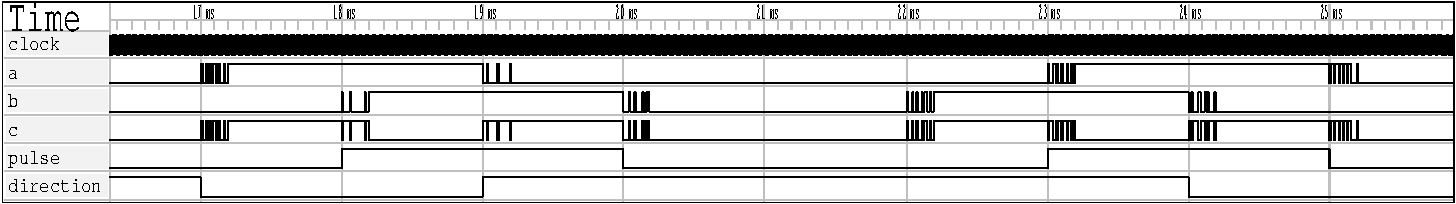
\includegraphics[width=\textwidth]{quadrature_decoder_gtkwave.pdf}
\caption{Waveforms from testbench, visualised by GTKWave}
\end{figure}
\begin{figure}
\centering
\begin{tikztimingtable}
A         & LLL N(A1)HHN(A2)L LLL LN(A3)HHN(A4) LLL \\
B         & LLL LN(B1)HHN(B2) LLL N(B3)HHN(B4)L LLL \\
C         & LLL LN(C1)HN(C2)L LLL LN(C3)HN(C4)L LLL \\
D         & HHH N(D1)LLLN(D2) HHH N(D3)LLLN(D4) HHH \\
E         & LLL N(E1)HN(E2)LL LLL LLN(E3)HN(E4) LLL \\
F         & LLL LLN(F1)HN(F2) LLL N(F3)HN(F4)LL LLL \\
Pulse     & LLL LN(P1)HHN(P2) LLL LN(P3)HHN(P4) LLL \\
Direction & LLL LLN(D1)H HHH HHN(D2)L LLL \\
\extracode
\begin{pgfonlayer}{background}
\draw[help lines] (A1) -- (E1);
\draw[help lines] (A2) -- (D1);
\draw[help lines] (A3) -- (P3);
\draw[help lines] (A4) -- (P4);
\draw[help lines] (B1) -- (P1);
\draw[help lines] (B2) -- (P2);
\draw[help lines] (B3) -- (F3);
\draw[help lines] (B4) -- (D2);
\end{pgfonlayer}
\end{tikztimingtable}
\caption{Clean waveforms}
\end{figure}
\begin{figure}
\centering
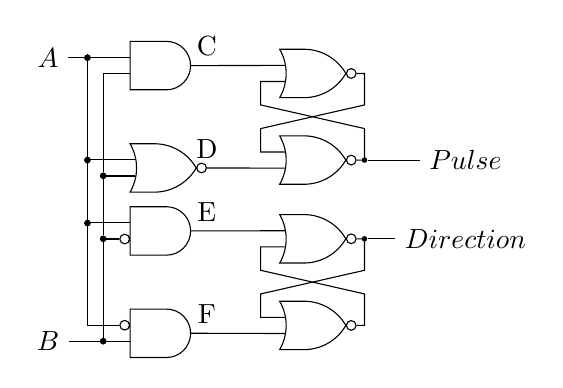
\begin{tikzpicture}[circuit logic US]
\node (A) at (0,1.8) {$A$};
\node (B) at (0,-1.8) {$B$};
\node[branch, draw] at ($(A)+(0.5,0)$) (A1) {};
\node[branch, draw] at ($(A1)+(0,-1.3)$) (A2) {};
\node[branch, draw] at ($(A2)+(0,-0.8)$) (A3) {};
\node[branch, draw] at ($(B)+(0.7,0)$) (B1) {};
\node[branch, draw] at ($(B1)+(0,+1.3)$) (B2) {};
\node[branch, draw] at ($(B2)+(0,+0.8)$) (B3) {};
\node[and gate, draw, inputs=ni] at ($(B2) +(0.7,+0.1)$) (And1) {};
\node[and gate, draw, inputs=in] at ($(B1) +(0.7,+0.1)$) (And2) {};
\node[and gate, draw, inputs=nn] at ($(A1) +(0.9,-0.1)$) (And3) {};
\node[nor gate, draw, inputs=nn] at ($(A2) +(0.9,-0.1)$) (Nor1) {};
\node[nor gate, draw, inputs=nn] at ($(And1) +(1.9,-0.1)$) (Nor2) {};
\node[nor gate, draw, inputs=nn] at ($(And2) +(1.9,+0.1)$) (Nor3) {};
\node[nor gate, draw, inputs=nn] at ($(Nor1) +(1.9,+0.1)$) (Nor4) {};
\node[nor gate, draw, inputs=nn] at ($(And3) +(1.9,-0.1)$) (Nor5) {};
\node (P) at ($(Nor4)+(2,0)$) {$Pulse$};
\node (D) at ($(Nor2)+(2,0)$) {$Direction$};
\draw (A) -- (A1);
\draw (B) -- (B1);
\draw (A1) -- (A2);
\draw (A2) -- (A3);
\draw (B1) -- (B2);
\draw (B2) -- (B3);
\draw (A3) |- (And1.input 1);
\draw (B2) |- (And1.input 2);
\draw (A3) |- (And2.input 1);
\draw (B1) |- (And2.input 2);
\draw (A1) |- (And3.input 1);
\draw (B3) |- (And3.input 2);
\draw (A2) |- (Nor1.input 1);
\draw (B3) |- (Nor1.input 2);
\draw (And1.output) -- +(0.2,0) node[above]{E} -- (Nor2.input 1);
\draw (And2.output) -- +(0.2,0) node[above]{F} -- (Nor3.input 2);
\draw (Nor2.output) -| node[branch] (D1) {} +(0.1,-0.4) -- ($(Nor3) +(-0.6,+0.4)$) |- (Nor3.input 1);
\draw (Nor3.output) -| +(0.1,0.4) -- ($(Nor2) +(-0.6,-0.4)$) |- (Nor2.input 2);
\draw (D1) -- (D);
\draw (And3.output) -- +(0.2,0) node[above]{C} -- (Nor5.input 1);
\draw (Nor1.output) -- +(0,0) node[above]{D} -- (Nor4.input 2);
\draw (Nor5.output) -| +(0.1,-0.4) -- ($(Nor4) +(-0.6,+0.4)$) |- (Nor4.input 1);
\draw (Nor4.output) -| node[branch] (P1) {} +(0.1,0.4) -- ($(Nor5) +(-0.6,-0.4)$) |- (Nor5.input 2);
\draw (P1) -- (P);
\end{tikzpicture}
\caption{Logic gate circuit}
\end{figure}
\begin{figure}
\centering
\begin{BVerbatim}
c <= a and b;
d <= a nor b;
e <= a and not b;
f <= b and not a;
dir <= dir_n nor e;
dir_n <= dir nor f;
pul <= pul_n nor d;
pul_n <= pul nor c;
pulse <= pul;
direction <= dir;
\end{BVerbatim}
\caption{VHDL code}
\end{figure}
\end{document}
